%% project_proposal_m_Panuco.tex
%% ---------------------------------------------------------------------------------------------------

\documentclass[12pt,journal,compsoc]{IEEEtran}

%-----PACKAGES-------------------------------------------------------------------------------------
 

% Copy package text here:
\usepackage{pdfpages}
\usepackage{graphicx}
\usepackage{algorithm}

% Formatting 30 minutes
% Research 2 hours
% Writing 5 hours
% Pages per hour - 1
% Need 8 Pages


%----- The DOCUMENT Environment-------------------------------------------------------------------

\begin{document}

\title{Bio-Informatics: Computer Science For Biological Modeling And Computation}

\author{Mario Panuco}


\date{\today}        % leaving the brackets empty omits the date
% To input the current date, you can type: \date{\today}

% The paper headers
\markboth{CSE185S: Bio-Informatics}%
{Panuco \MakeLowercase{\textit{et al.}}: CSE185s}

% this:
\IEEEpubid{0000--0000/00\$1738.00~\copyright~2007 IEEE}



\maketitle

%----- The SECTION Environment -------------------------------------------------------------------

\begin{abstract}
Bio-Informatics is a relatively young scientific field, that in many ways, is still searching for it's identity. It's applications can change the way medicine and epidemiology affects everyone's daily life. There are also applications of the field to things that don't directly affect most lives, but instead are meant to analyze ecosystems for the purpose of conservation and research. 

\end{abstract}
\IEEEPARstart{C}{omputer} science has found a way into almost every modern industry and science. Bio-informatics is one of the fields that has blended two sciences in a powerful way, where both biologists and computer scientists have the opportunity to collaborate and contribute through a mutual scientific language. This new scientific language has a promising future as both fields innovate and collaborate on applications of computer science to biological systems.  
\section{Introduction}

\subsection{Purpose}
The purpose of this paper is to present a cursory overview of bio-informatics and its growing importance.

The purpose of the project is to educate other UCSC STEM students on the basics of bio-informatics and the importance of bio-informatics in the modern-world. I hope the students learn to expand their knowledge base on the limits of science and get inspired to apply their skills to other fields outside their major.

\subsection{Intended Audience}
The intended audience for this project is an undergraduate student with rudimentary knowledge of computer science and/or biology.

\subsection{Style Guide}
I will be styling my in \LaTeX\ document according to the IEEE standards.

\tableofcontents

\clearpage

\section{Origins of Bio-Informatics}

The first baby-steps for bio-informatics encompassed creating databases for large data-sets and libraries of sequenced data. The first major data-set breakthrough was Dr. Margret Oakley's protein sequence database, which was created using computational models, entirely programmed on punch cards in FORTRAN (see Figure 1 for example).
\begin{figure}[H]
    \centering
    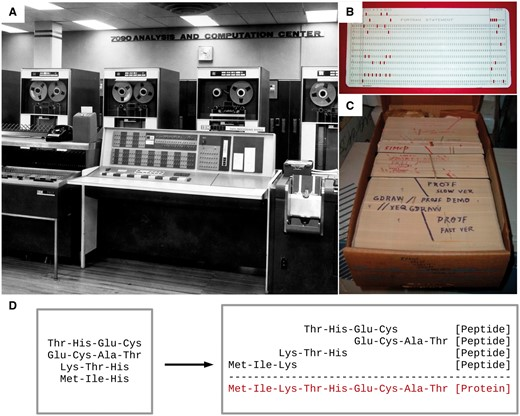
\includegraphics[width=\linewidth]{images/m_bby063f2.jpeg}
    \caption{Picture of IBM computer running FORTRAN code from a punch card for protein sequencing}
    \label{fig:FORTRAN Code}
\end{figure}

After the release of Oakley's book on protein sequencing, \emph{The Atlas Of Protein Sequence and Structure}, the infant bio-informatics community continued with improving on protein computation models. \\  
In the 1970s the field started to focus more on DNA sequencing because of a new idea, now referenced as the "Central Dogma" in molecular biology. The effect was that scientists focused on developing cheap and efficient methods for computing DNA sequencing as a means to protein sequencing. For example in 1970, the first dynamic programming algorithm for pairwise alignment was developed. The algorithm was developed for pairwise protein alignment because the focus of the field during the time was on protein sequences.  \cite{Gauthier2018}. From protein and DNA sequencing, the field started to research and develop solutions to more complex problems presented by its sister field, molecular biology, such as analyzing complete genomes. \\
These methods of DNA and protein sequencing formed the foundation of bio-informatics, until the 2000s, where Bio-Informatic scientists were presented with a new issue pertaining to the management and structuring of big data being collected by Bio-Informatic research and computations. This is still an ongoing issue and is anticipated to remain as an issue as long as data remains integral to Bio-Informatic. Modern research and methods focus less on sequencing and more on modeling whole organisms and biological ecosystems.


\section{Hidden Markov Models}
\subsection{Background on Hidden Markov Models}
The discovery of Hidden Markov Models (HMMs) as an efficient tool for problems such as gene prediction, sequence classification, and alignment of sequences propelled Bio-Informatics. HMMs are considered a Markov process, similar to a Markov-Decision-Process, which are used in fields like artificial intelligence as means of making reasonable predictions. HMMs are found to be an intuitive mathematical representation of biological systems. \cite{7530222} \\
HMMs in isolation don't perform Bio-Informatic computation, the model simply serves as the mathematical model used to represent and manage bio-informatic problems such as multiple sequence alignment, genome mapping, and genome prediction.

\subsection{Model of a Hidden Markov Model}
Hidden Markov Models assume that the observations used for observation probability come from underlying "hidden" states, rather than the state of our model. \\ \\
The model can be defined by 3 components for $N$ states: \\
Set of state transition probabilities $T$: Probability $P_ij$ for state $S_i$ and state $S_j$ \\
Set of observation emission probabilities $O$ - Probability of seeing observation $O_k$ while in state $S_i$ \\
State initialization probability $P(\lambda | S_i)$: The probability of our HMM $\lambda$ occurring in state $S_i$ \\

Figure 1 presents an example of a HMM that relates the number of ice cream eaten with the weather of the day. In the example, $B_1$ and $B_2$ are the observation emission probabilities, the state transition probabilities are the connections between the hot and cold observations, and the state initialization probability is the octagon at the bottom. The state initialization probability in the example shows that more ice cream is eaten on hot days \cite{Standford_HMM_Notes}.
\begin{figure}[H]
    \centering
    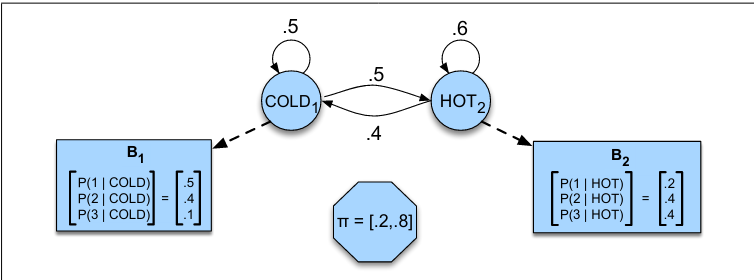
\includegraphics[width=\linewidth]{images/Screenshot 2022-06-07 at 18-31-01 A.pdf.png}
    \caption{Hidden Markov Model}
    \label{fig:Hidden Markov Model}
\end{figure}


\subsection{HMM Algorithms}
Within this field, there are numerous applicable algorithms that utilize HMMs, each with their own purpose and efficiency. To help conceptualize the application of these models to Bio-Informatics, it's important to understand the formal math behind HMM algorithms. More specifically, I wanted to introduce the evaluation problem for HMMs.

\begin{center}
    The evaluation problem for HMMs means we are trying to find the probability of a set of observations O given an HMM $\lambda$ \\
    \begin{math} P(O\vert \displaystyle \lambda)=\sum_{S}P(O\vert S;\lambda).(S\vert \lambda)
    \end{math}
\end{center}

Now that we have defined the evaluation problem, we can present the "Forward Algorithm" for the evaluation problem. The algorithm begins its computation at the start of a sequence and finds the probability of a certain observation/genome sequence at each step.
\begin{center}

    Forward Algorithm for the state where we see those observations
    \begin{math} \delta_{K}(u)=P(e_{1},.\ldots.,e_{K};S_{K}=u\vert \lambda)
    \end{math}
    
\end{center}

\section{Dynamic Programming In Pairwise Alignment}
A fundamental computer science concept for Bio-Informatics is dynamic programming. Most computer science students are initially introduced to this problem-solving technique in their algorithms classes (at UCSC this class is CSE 102). It's a fundamental tool, and is often evaluated during computer science interviews. This technique has found its way into numerous computer science subfields like artificial intelligence and Bio-Informatics. \\
For Bio-Informatics it's used as a way to efficiently compute pairwise alignment. Dynamic programming works by utilizing recursion and memoization to break down the problem into smaller chunks, until there are no more dependencies to other cells in the memoization table.

\subsection{Needleman-Wunsh Algorithm}
The Needleman-Wunsh algorithm is the basic algorithm for pairwise alignment using dynamic programming. The algorithm utilizes an $N X N$ memoization table to store the currently misaligned sequence. Each cell in will represent a value for match, mismatch, or gap. The chain of dependencies start at the cell $i=1, j=1$, which is the value we want if we wish to know if the sequences are aligned, and the computation of a cell's value is recursively called the cell that requires its dependency. This continues until we reach $i=N, j=N$, where the cell no longer depends on another cell's value. The algorithm then backtracks back to $i=1, j=1$, filling the memoization table along the way and clearing dependencies.

\subsection{Issue With Dynamic Programming}
The main issue with dynamic programming for large data-sets is the bottleneck that comes with how interacting with large memory works on modern computers. To combat this Bio-Informatic scientists are designing frameworks that adjust the current use of dynamic programming to more efficiently interact with the memory on computer systems, specifically by introducing cache-oblivious algorithms for pairwise alignment. \cite{4609376} \\ 
Dynamic programming allows for efficient computation over large data-sets and models. The key idea of dynamic programming is that a state depends on the values of other adjacent or related states, so you start the algorithm at a state that has no dependencies and from there build the model of states until you have successfully computed every necessary state. \\ 
As a result of continuous research into algorithms, such as dynamic programming, for genome sequencing, the cost of whole genome sequencing has decreased past Moore's law, as illustrated by figure 3 \cite{genome.gov_2021}.
\begin{figure}[H]
    \centering
    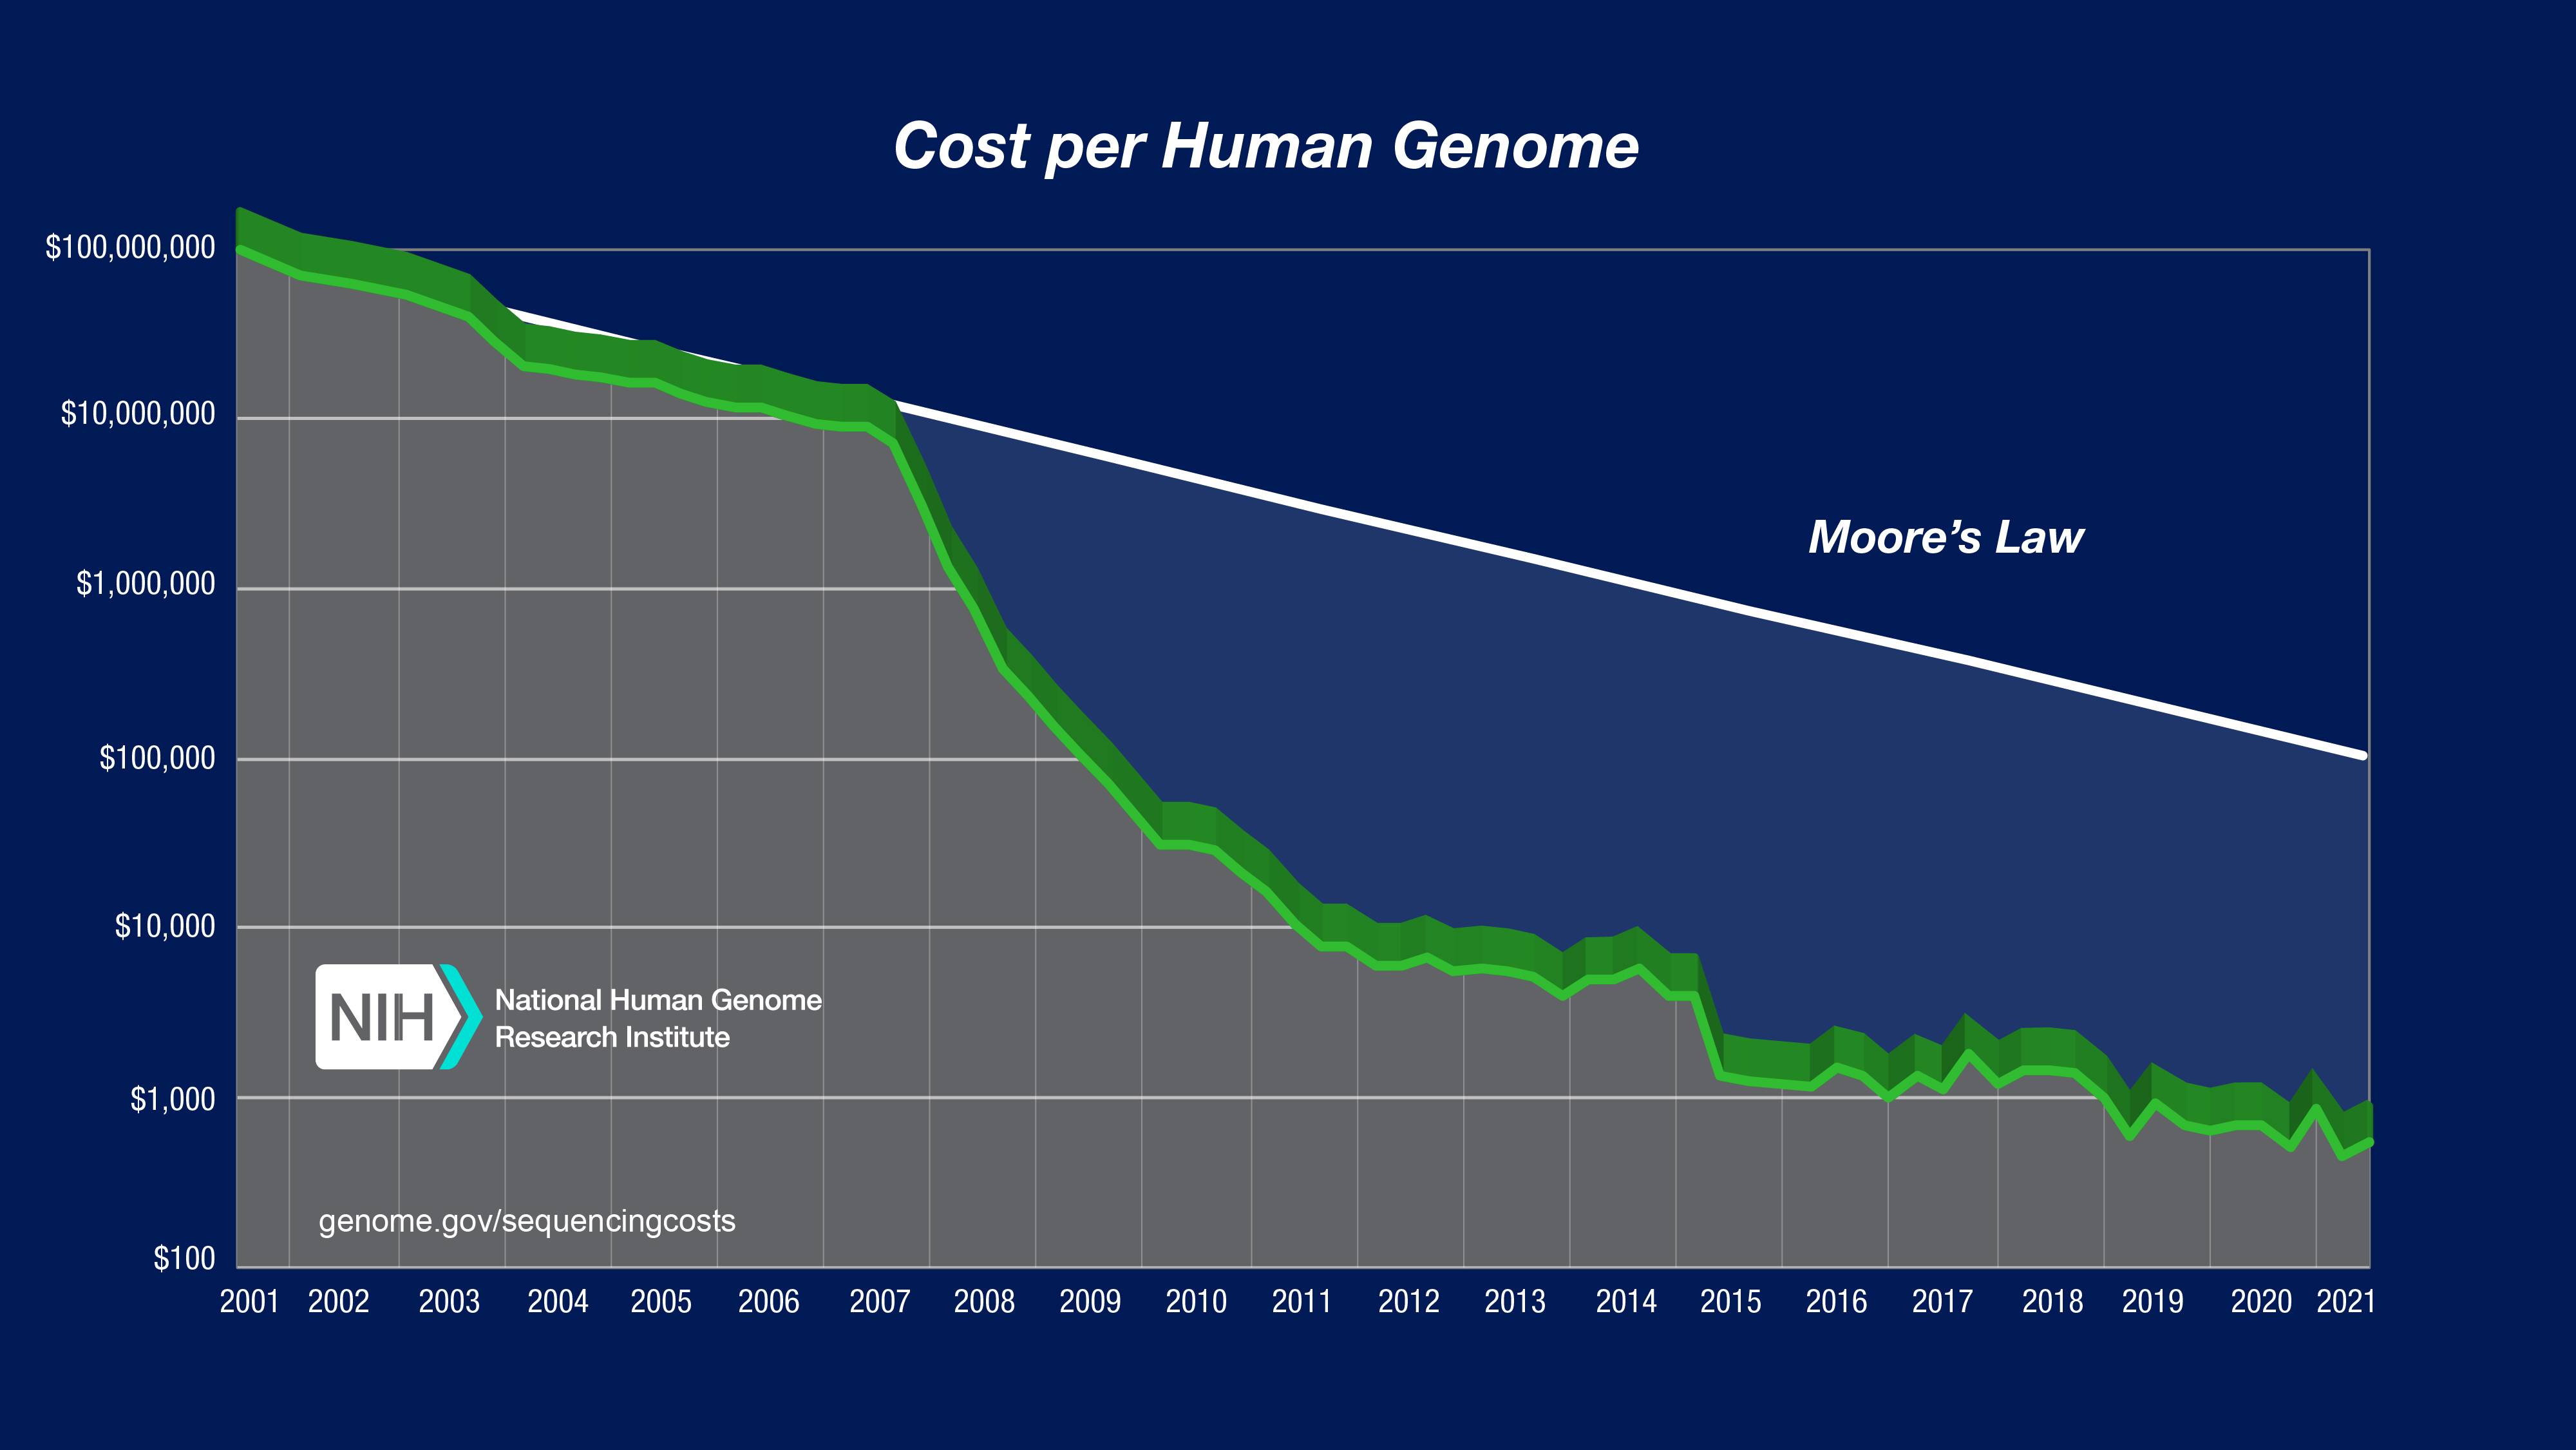
\includegraphics[width=\linewidth]{images/2021_Sequencing_cost_per_Human_Genome.jpg}
    \caption{Cost Human Genome}
    \label{fig:Cost Human Genome}
\end{figure}

\section{Genomic Epidemiology Applications and Research}
Protein and DNA sequencing has brought us to modern genome sequencing, the basis for genomic epidemiology. Genomic epidemiology works by using whole genome sequencing to sorting whole genome sequences, by targeting specific sections of the sequence for similarity. For infectious diseases, those with similar sequences are cases originating from the same outbreak. This can be used to find the outbreak of new strains, as well as which the main strain's stake in new cases. Genomic epidemiology is also applicable to cancer prediction and prevention \cite{Kitano2013}.

\subsection{COVID-19}
According to the World Health Organization as of May 29th 2022, the COVID-19 pandemic has affected 213 countries, over 526 million cases, and over six million deaths. As a result, there's been an effort to utilize genomic epidemiology for COVID-19 drug development, early detection, and prediction. With these new computation methods, there's hope to be able to more accurately predict the pandemic and mitigate vulnerabilities when they are observed.  

\subsection{Case Study: BeCaked}
Deep learning and genomic epidemiology can be combined to more efficiently predict COVID statistics. The motivation for this is to notify the public of possible massive outbreaks in their area. This also helps researchers determine how new COVID-19 strains are spreading in counties. 

The BeCaked project was created with the goal of creating an explainable AI that accurately forecasts COVID-19 statistics\cite{Nguyen2022}. The training data that's fed into the machine learning model comes from John Hopkins University. The data set contains data for susceptible, infectious, recovered, and dead cases. It's important to include susceptible because if we are predicting the COVID-19 rate in a county with a higher average age, we need to associate a susceptible statistic because the model should behave differently for this county compared to a county with different demographics and age. \\
This formal representation of a model in the project was based on the data, the researchers call this the SIRD model (see Figure 4. There are edge cases to this model, as seen in figure , where more recovered cases affect your model's susceptible value.

\begin{figure}[H]
    \centering
    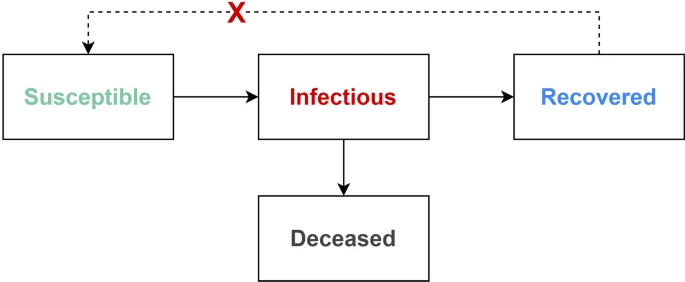
\includegraphics[width=\linewidth]{images/Screenshot 2022-06-07 at 21-30-50 BeCaked An Explainable Artificial Intelligence Model for COVID-19 Forecasting - Scientific Reports.png}
    \caption{SIRD Model}
    \label{fig:SIRD Model}
\end{figure}

The deep learning model comes in the form of a $N * 4$ matrix, where $N$ is the number of days we are training our model on. The $j$ row of the matrix is length 4 because that is our model's data for each day $i$. The results of BeCaked showed that it was accurate up to a 0.012 mean absolute percentage error at the global prediction level. The accuracy of the model was lower for modeling at the country level. This is a result of countries being open systems, as in they are affected by outside factors that can't be observed in a country's model. The global model is completely closed and isolated by external factors that affect COVID-19 statistics.
\subsection{Importance Of This Research}
I think it's important to establish importance on the fact that COVID prediction, biodiversity prediction, and other prediction-based Bio-Informatic problems can and should be tools used by legislators and those with power over these systems when they make decisions.  

\section{Applications of Bio-Informatics}
Bio-Informatics is a very new and modern field, whose parent fields are either just as new, in the case of computer science, or constantly evolving new scientific methods and applications, in the case of biology. The uncertainty of this new field means there's no prediction on how applicable bio-informatics will be to our daily lives in 50 years. The field could reach a bottleneck or deadlock of what it's limits or it could maintain its growing rate and its applications could drastically change the way humans live. The current possible applications for bio-informatics are: genome sequencing, medical diagnosis, modeling of biological systems for the the purpose of analyzing bio-diversity and other aspects of a biological system, and genome data-collection for the purpose of analyzing variation and accuracy of models. 

\subsection{Medical Diagnosing}
Medical diagnosing works very similarly to other prediction models for Bio-Informatics such as genomic epidemiology prediction. Using a person's whole genome sequence, we can search for genomes that are precursors or indicators of diseases. Along with diagnosing, this same concept is applicable to finding personalized cures and medicine based on a person's whole genome sequences. The figure below demonstrates a basic model for applying machine learning for the purpose of cancer prediction/susceptibility in a person's genome sequence.
\begin{figure}[H]
    \centering
    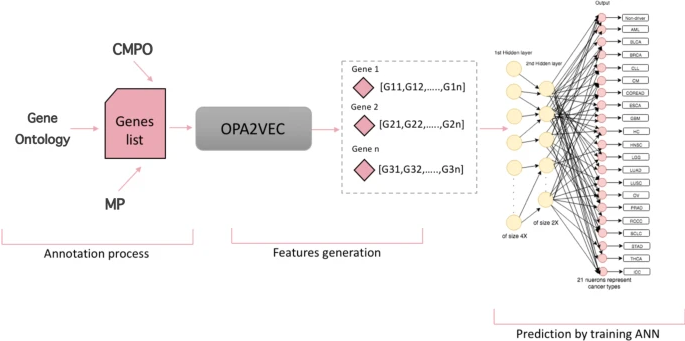
\includegraphics[width=\linewidth]{images/Screenshot 2022-06-07 at 23-00-03 Ontology-based prediction of cancer driver genes - Scientific Reports.png}
    \caption{Workflow Model For Cancer Prediction}
    \label{fig:Workflow Model For Cancer Prediction}
\end{figure}
In this specific model, the gene list is fed into OPA2VEC as a way to extract features from the genomic data\cite{Althubaiti2019}. A large portion of the application of machine learning for the purpose of cancer diagnosing comes from the ability to extract useful features that can be replicated across different genome data from multiple patients with the same form of cancer or similar genetic encoding. These features are necessary in order to train, analyze, and fine tune the cancer prediction model for accuracy.

\subsection{Drug Discovery And Testing}
Bio-Informatics for drug discovery works by using machine learning to create accurate alignments of phenotypic gene expressions. This process significantly reduces the amount of possible chemical combinations that can be used to create drugs that then go into clinical trials. 
\begin{figure}[H]
    \centering
    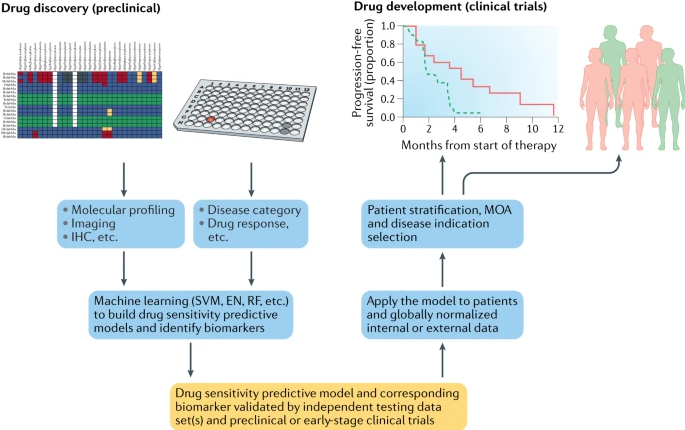
\includegraphics[width=\linewidth]{images/Screenshot 2022-06-07 at 23-54-30 Applications of machine learning in drug discovery and development - Nature Reviews Drug Discovery.png}
    \caption{Machine Learning For Drug Discovery}
    \label{fig: Machine Learning For Drug Discovery}
\end{figure}
The above figure shows the workflow of drug discovery. It's important to not that drug discovery doesn't do all the computation needed to find useful and side-effect free drugs. 
\section{Privacy Concerns}
As this technology improves, it's important to be conscious of the possible exploitative avenues this science can bring. Bio-Informatics is in the same case as other new technologies, like image recognition; this technology can be invasive and instinctively serve as data-collection mines. As illustrated by figure 6, the ownership of genome data can be transferred or owned by multiple entities, such as a genome research center and local authorities.

\begin{figure}[H]
    \centering
    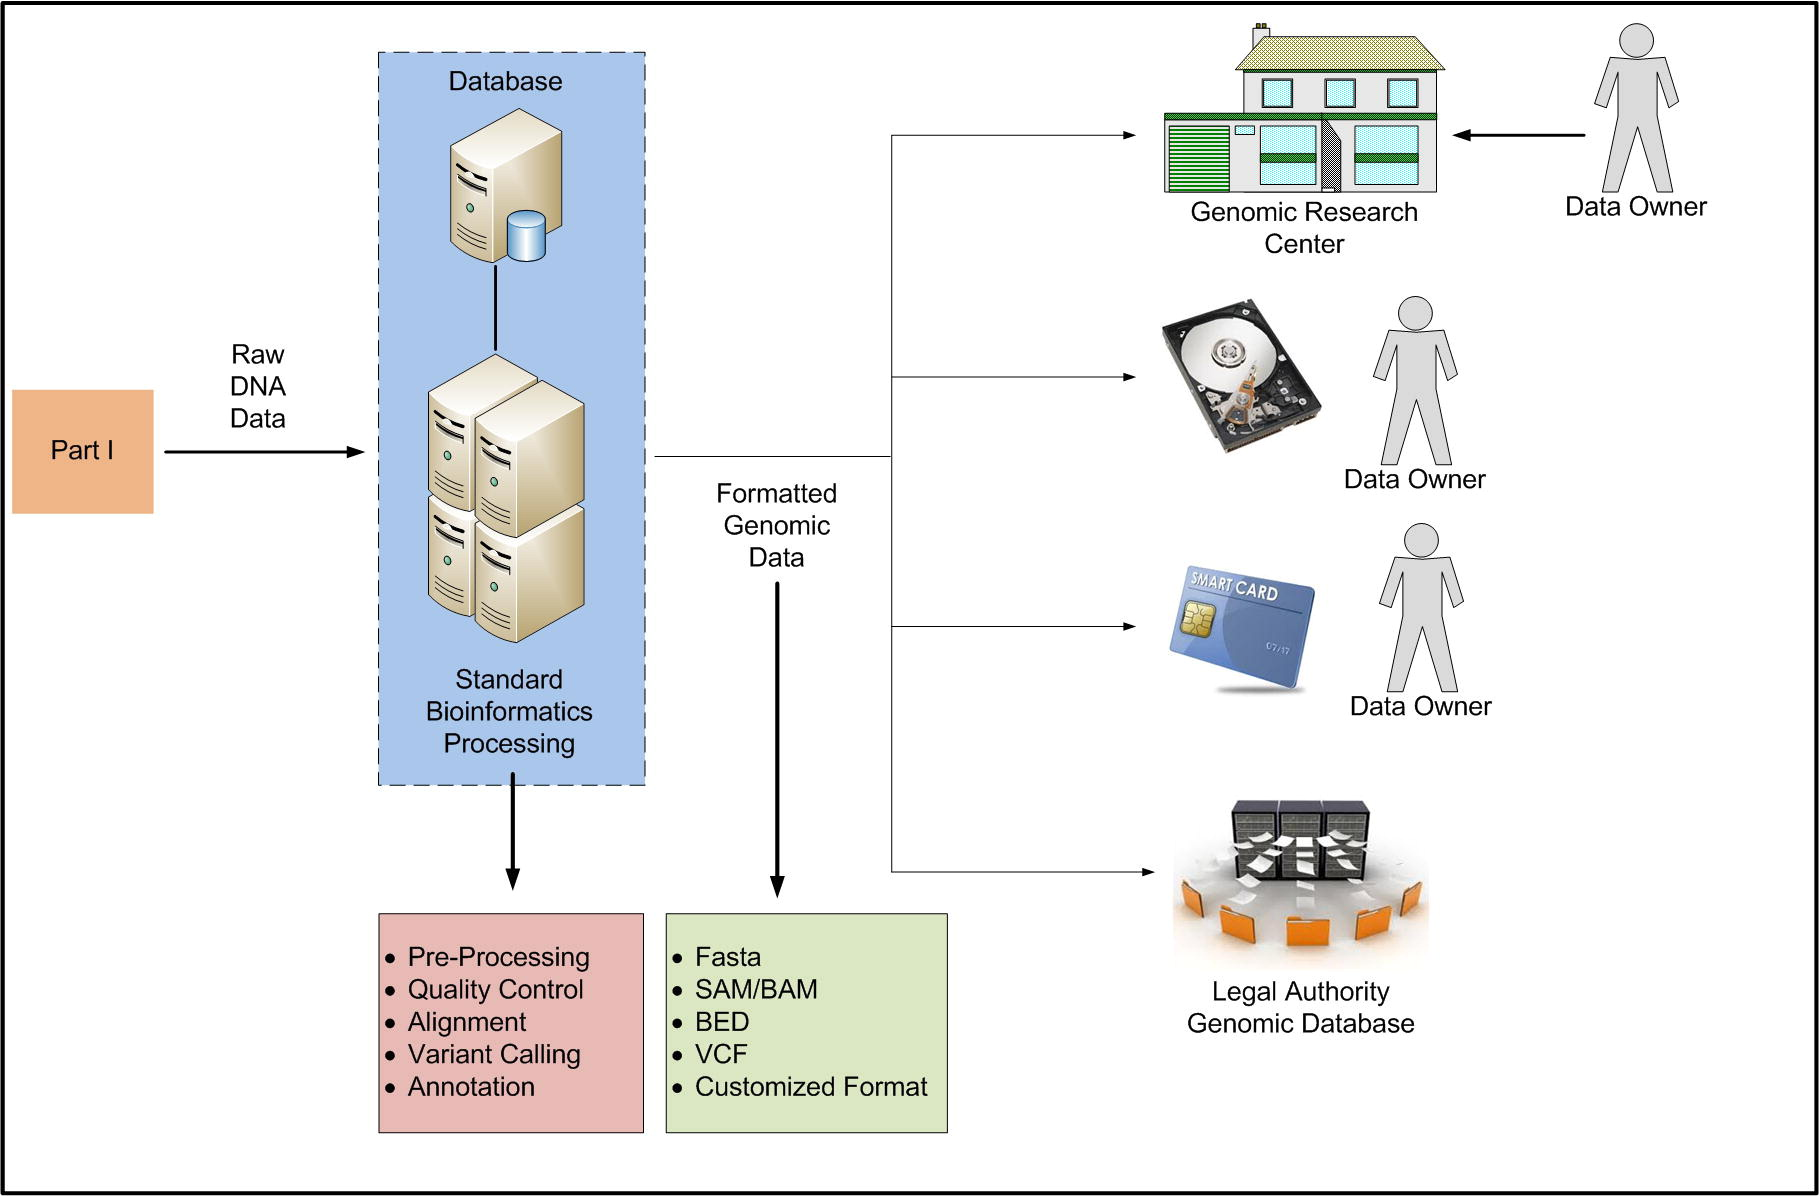
\includegraphics[width=\linewidth]{images/1-s2.0-S1532046415001100-gr2b_lrg.jpg}
    \caption{Flow Of Bio-Informatic Data}
    \label{fig:Flow Of Bio-Informatic Data}
\end{figure}

The biggest concern for privacy comes with governments keeping collections of personal genome data, for the purpose of policing and surveillance. For example in 2018, genome data used in a genetic ancestry test was given to the police. This data was used to convict Joseph James DeAngelo of crimes committed by a serial killer of the name "Golden State Killer" that committed at least 13 murders between 1974 and 1986.

\subsection{Solutions}
Solutions to this issue mostly come in the form of creating and introducing more security-enhancing technology to data collections at the infrastructure level. This solution is not enough to ensure privacy of your biological data, which is why there's been a growing number of legislation of data-privacy. As this field continues to grow and as genome data collections expand their data set, there's going to be a need for standardized human rights laws to protect data-privacy across countries.

\section{Biodiversity Informatics}
Biological systems in nature are rich in data, which means the data is impossible to process by just humans. This is where Bio-Informatics is stepping in. With the help of computers, biologists are able to see the true picture of their data and analyze the health of biological systems.

The introduction of these new analytical tools help, not only biologists, but those with direct authority over conservation and wildlife. The ability to have open and clear indicators of an ecosystem's health and condition in specific areas like: taxonomy, invasive species, and effects of the global environment system on the ecosystem.
\subsection{Ecological Niche Modeling}
Ecological Niche Modeling (ENM) is a model used to predict the distribution of species over a geographical area. This is important when it comes to surveying the health of an area because it helps research pin down on vulnerable areas for species or on areas that have a newly introduced invasive species that is disrupting the natural organization of the ecosystem. This following figure shows the different features that come into play when analyzing biodiversity and the status of a regions biodiversity health. 
\begin{figure}[H]
    \centering
    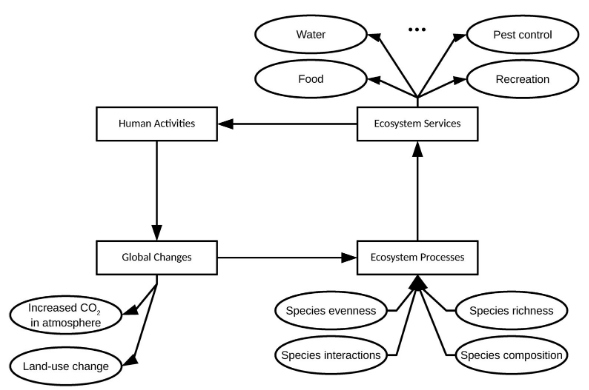
\includegraphics[width=\linewidth]{images/Screenshot 2022-06-07 at 23-24-05 A survey of biodiversity informatics Concepts practices and challenges - widm.1394.png}
    \caption{Ecosystem connection to outside features and conditions}
    \label{fig:Ecosystem connection to outside features and conditions}
\end{figure}
It's important to keep these external features in mind when creating layers and models for ENM because neglecting the fact that an ecosystem is not a closed system will introduce chaos into the model and ruin predictions for a species' distribution and health within the ecosystem.  \\ 

The main factors that affect a species probability of existence in a region are abiotic conditions, biotic conditions, and dispersal capacity. Abiotic conditions are environmental conditions like rainfall measurements and temperature. Biotic conditions are interactions between the species and other biology in the environment, e.g. the ratio between our target species and one of its predator species. Bio-Informatic researchers currently focus more on abiotic conditions because they have produced the best accuracy for ENMs. \cite{ctx28867828220006531}
An example of layers that could go into an ENM model is illustrated in figure 8 \cite{hallman_robinson_2020}. To make the ENM in the figure more complex, a designer could introduce a new biotic layer for regions with trees taller than a certain height, which is a suitable habitat for a predator bird species to our subject species.

\begin{figure}[H]
    \centering
    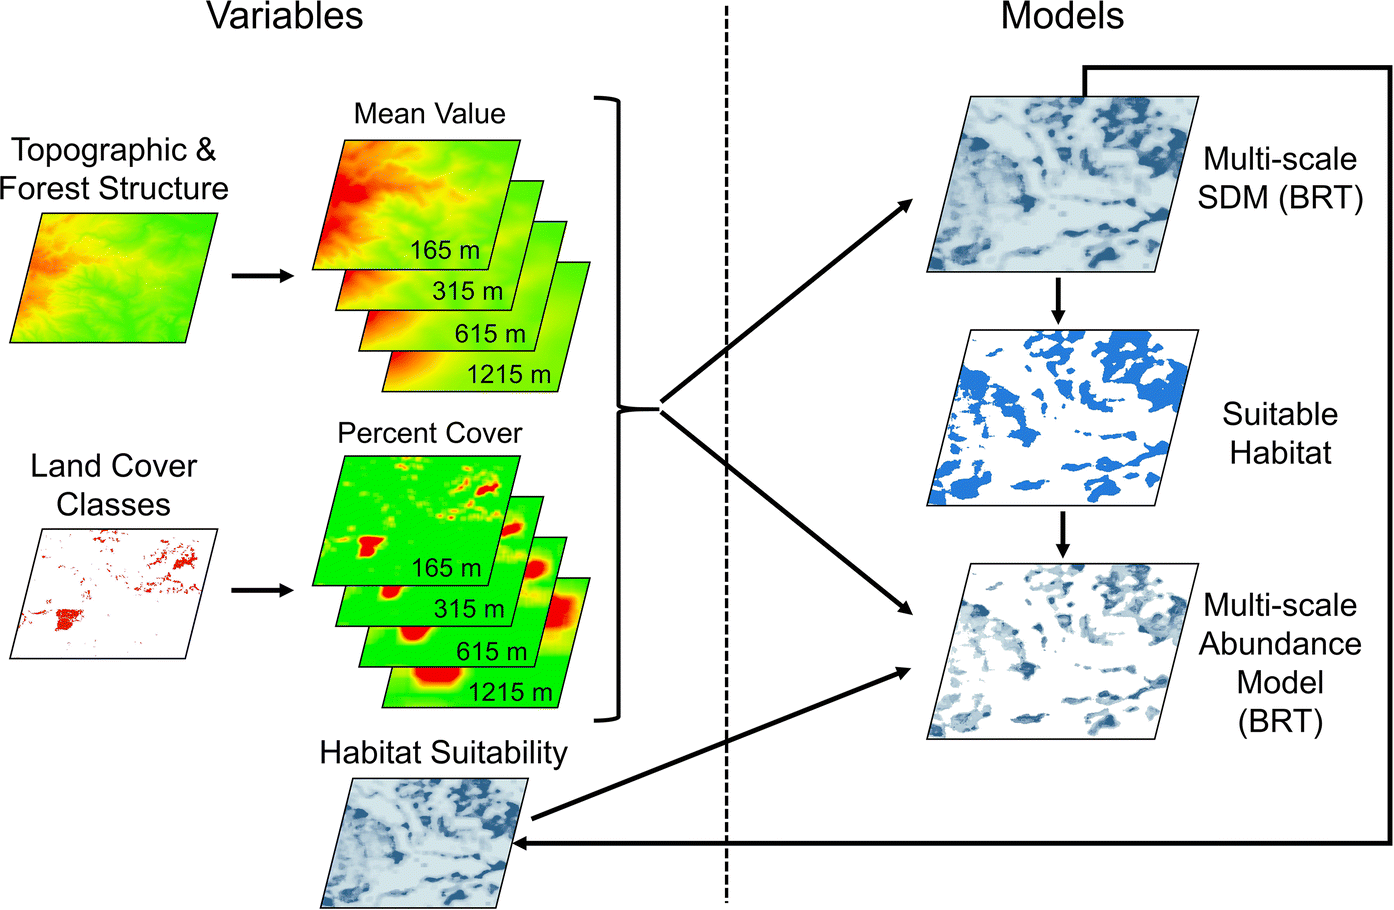
\includegraphics[width=\linewidth]{images/10980_2020_1007_Fig1_HTML.png}
    \caption{Example of Layers in an ENM}
    \label{fig:Example of Layers in an ENM}
\end{figure}

This process of using ENMs for biodiversity informatics is split into three steps: preprocessing, modeling, and postprocessing. The preprocessing stage deals with selecting which data is important for the ENM, retrieving said data, and then filtering the data for noise. The modeling stage is where computational models are applied to the previously curated data. There are many different computational methods that can be applied during the modeling phase such as machine learning algorithms like Maxent. The post-processing phase consists of retrieving the actual model projection from our machine learning and evaluating such projection.

The more complex and biodiverse our subject environment is, the more difficult it is to create an accurate model of the system for use of ENMs.

\section{Conclusion}
Bio-Informatics is a rich scientific field that continues to progress and bloom. Computer science has proven to be invaluable for processing and modeling biological data, a shortcoming of biology before bio-informatics, for the purposes of biodiversity, epidemiological research, medical diagnosing, and cancer prediction. As we move into the future, we will see parallel progression between computer science, Bio-Informatics, as well as fields like biomolecular engineering.

%----- ACKNOWLEDGEMENT SECTION -------------------------------------------------------------------
% Explain what the asterisk * does in the next line:
\section*{Acknowledgements}
\label{Textbook}
I would like to thank Richard Durbin, Sean R. Eddy, Anders Krogh, and Graeme Mitchison for their work on the textbook Biological sequence analysis [1]. The book is what initially sparked my interest in bio-informatics.
I would also like to thank overleaf for their \LaTeX\ software, which was used to edit and compile this document.

%----- BIBLIOGRAPHY ------------------------------------------------------------------------------

\bibliographystyle{plain}
\bibliography{references.bib}

%----- Optional: BIOGRAPHY Section ---------------------------------------------------------------
 
\vfill
\begin{IEEEbiography}[{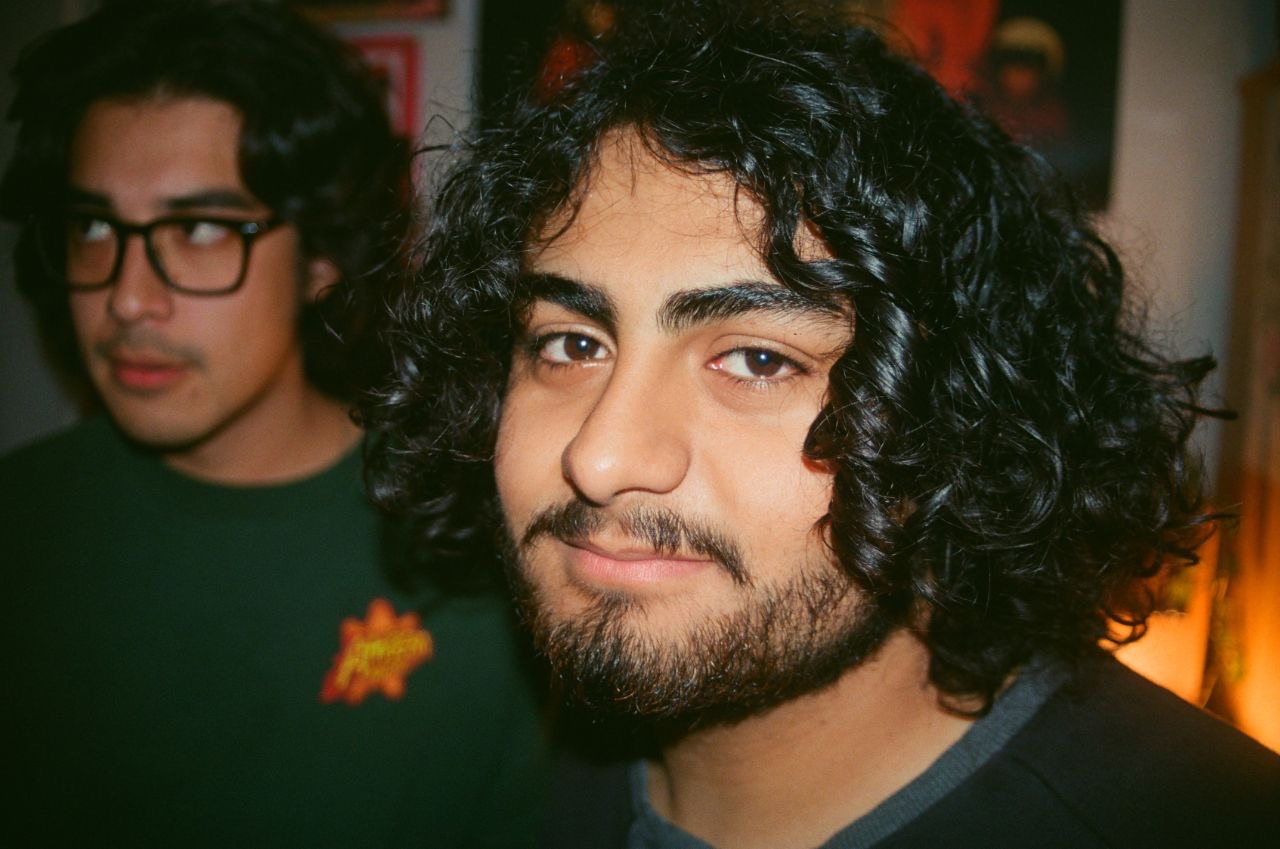
\includegraphics[width=1in,height=1.25in,clip,keepaspectratio]{headshot.jpg}}]{Mario Panuco}
I'm a Junior computer science student at the University of California, Santa Cruz. My favorite fields within computer science are assistive technology, machine learning, bio-informatics.
\end{IEEEbiography}

\end{document}



